\Chapter{Általános információk (?)}

Ebben a fejezetben néhány általános információ található, amik a dolgozat teljes egészére érvényesek.

\Section{Felhasznált képek}

A teszteléshez csendéletekről készült képeket gyűjtöttem az unsplash nevezetű weboldalról. \cite{unsplash}
A csendéleteken a tárgyak intenzitása jól elkülönül a háttér intenzitásától így egyszerűbben lehet rajta szegmentálást végrehajtani.
A képek a \ref{fig:images}. ábrán láthatóak, a neveik a 0 és 5 közötti számok, pl. 0.jpg.

\begin{figure}[htb]
    \centering % <-- added
\begin{subfigure}{0.25\textwidth}
  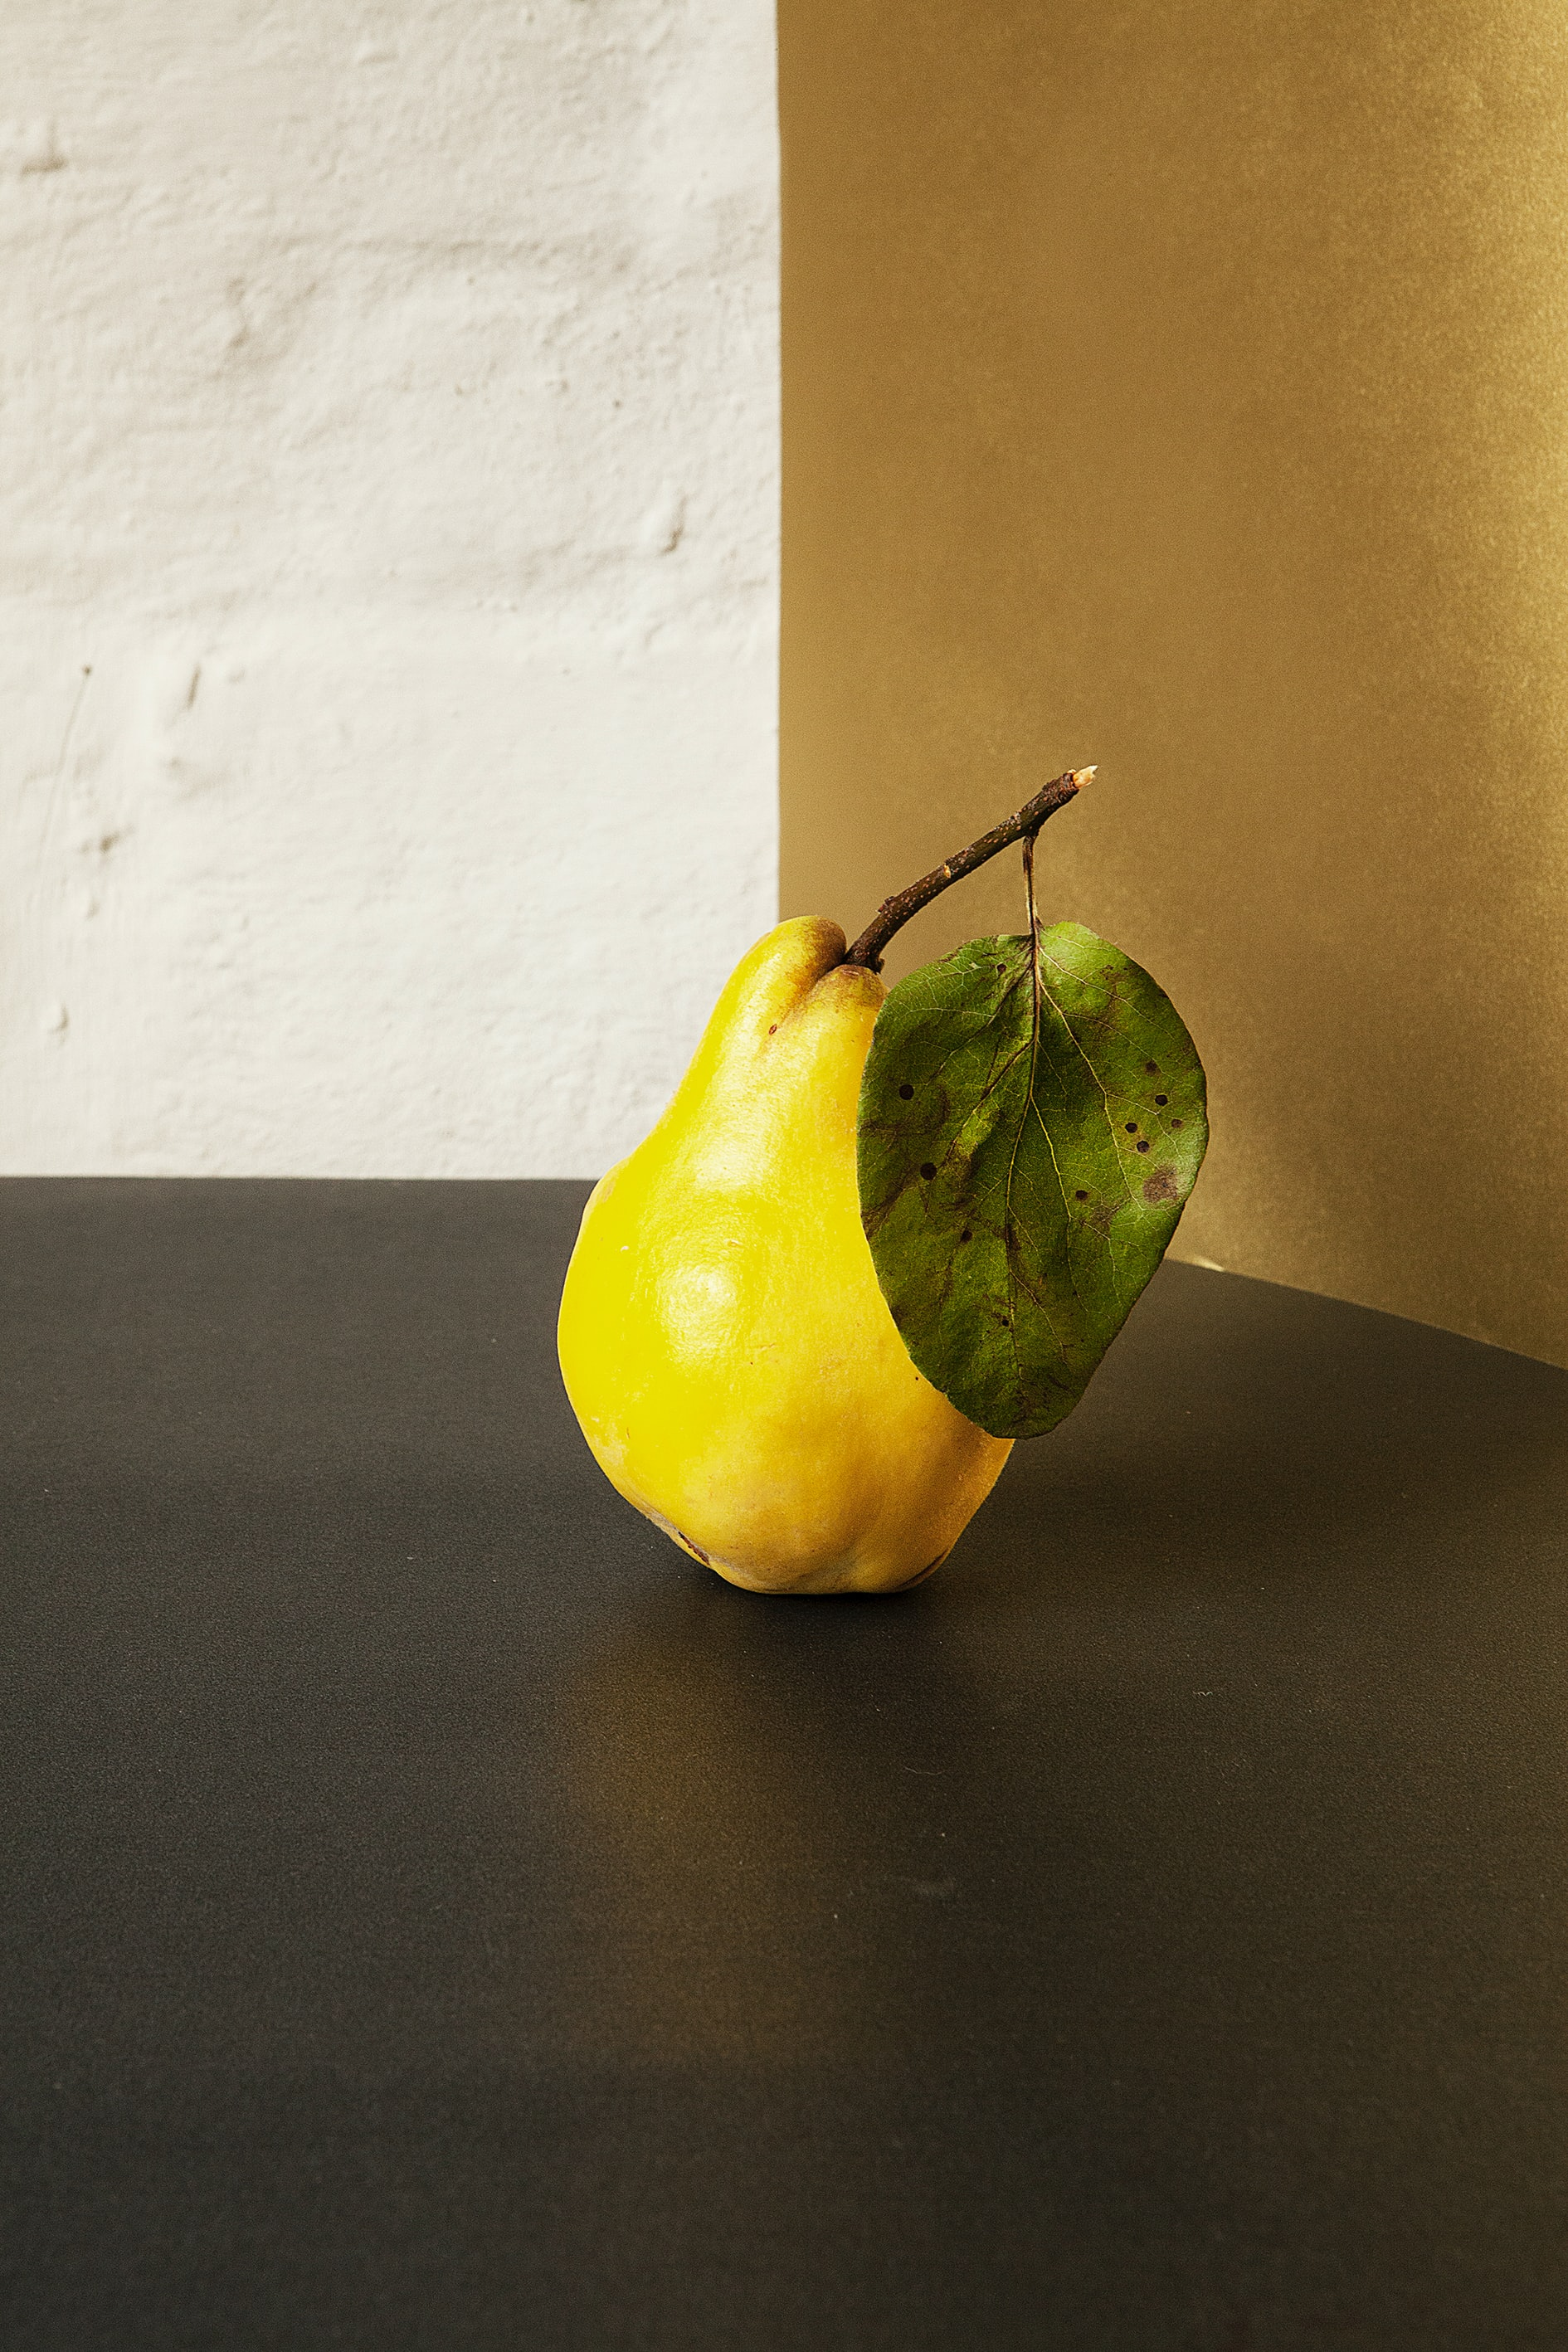
\includegraphics[width=\linewidth]{../images/0.jpg}
  \caption*{0.jpg}
  \label{fig:0jpg}
\end{subfigure}\hfil % <-- added
\begin{subfigure}{0.25\textwidth}
  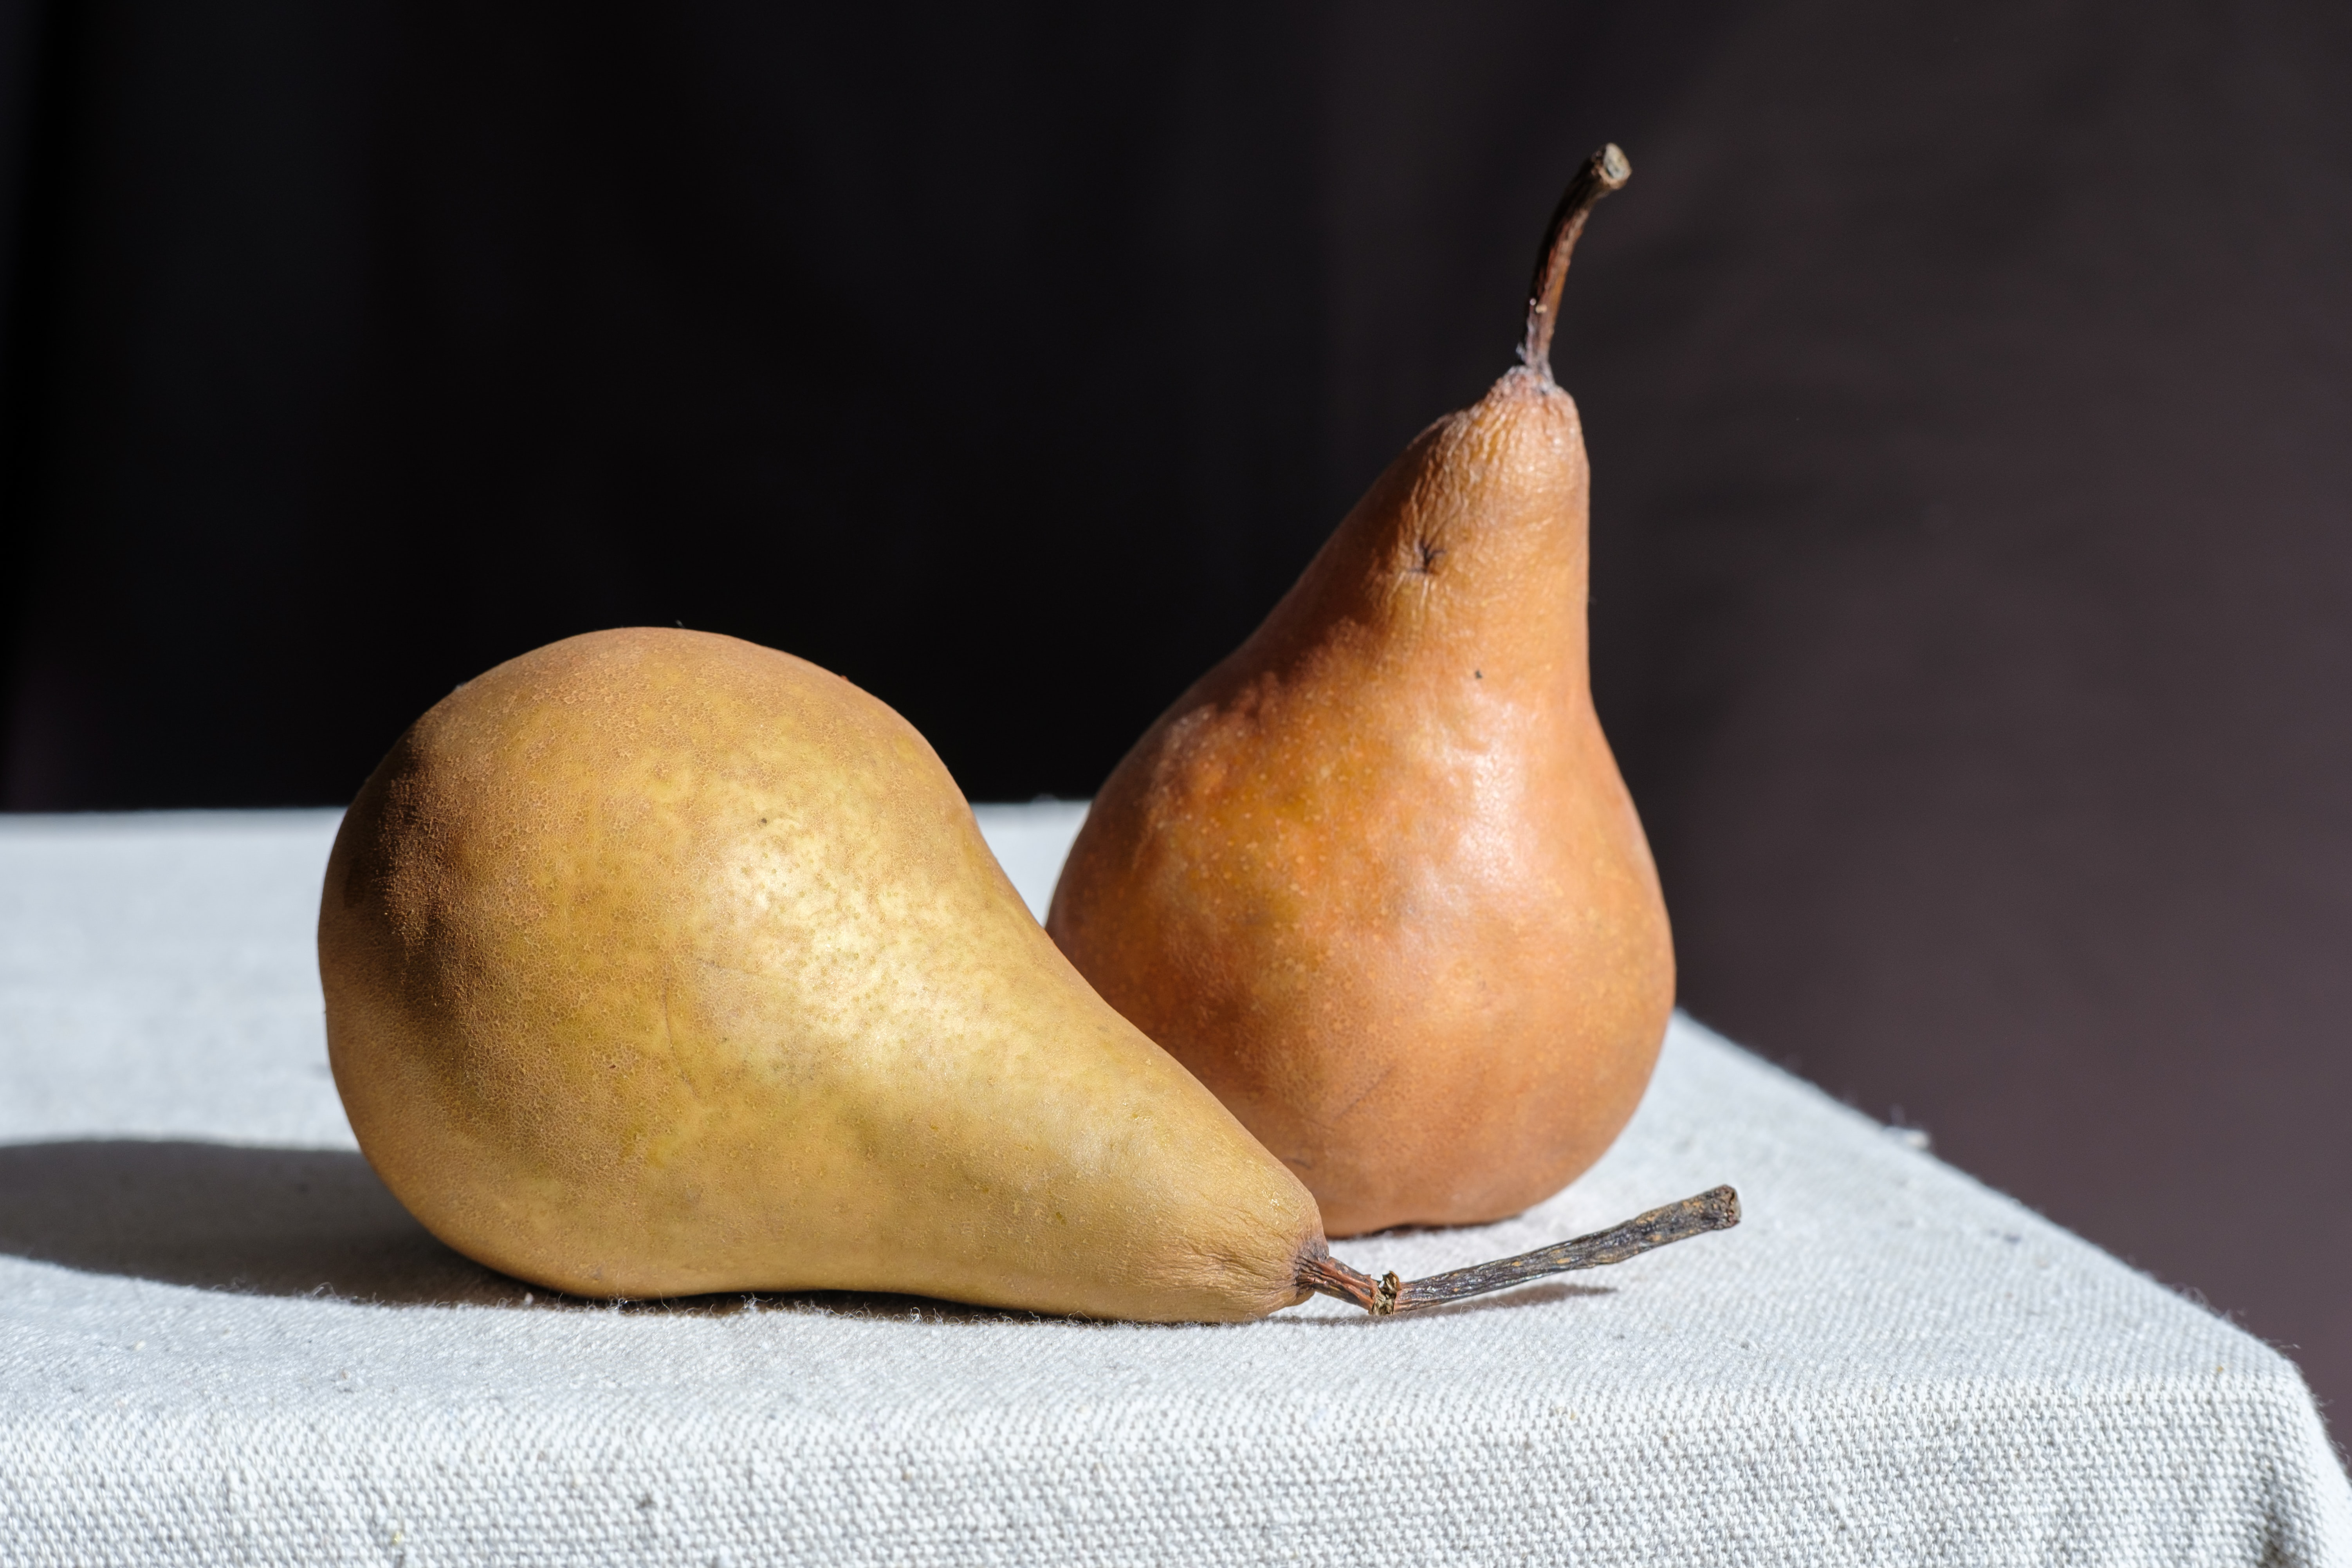
\includegraphics[width=\linewidth]{../images/1.jpg}
  \caption*{1.jpg}
  \label{fig:1jpg}
\end{subfigure}\hfil % <-- added
\begin{subfigure}{0.25\textwidth}
  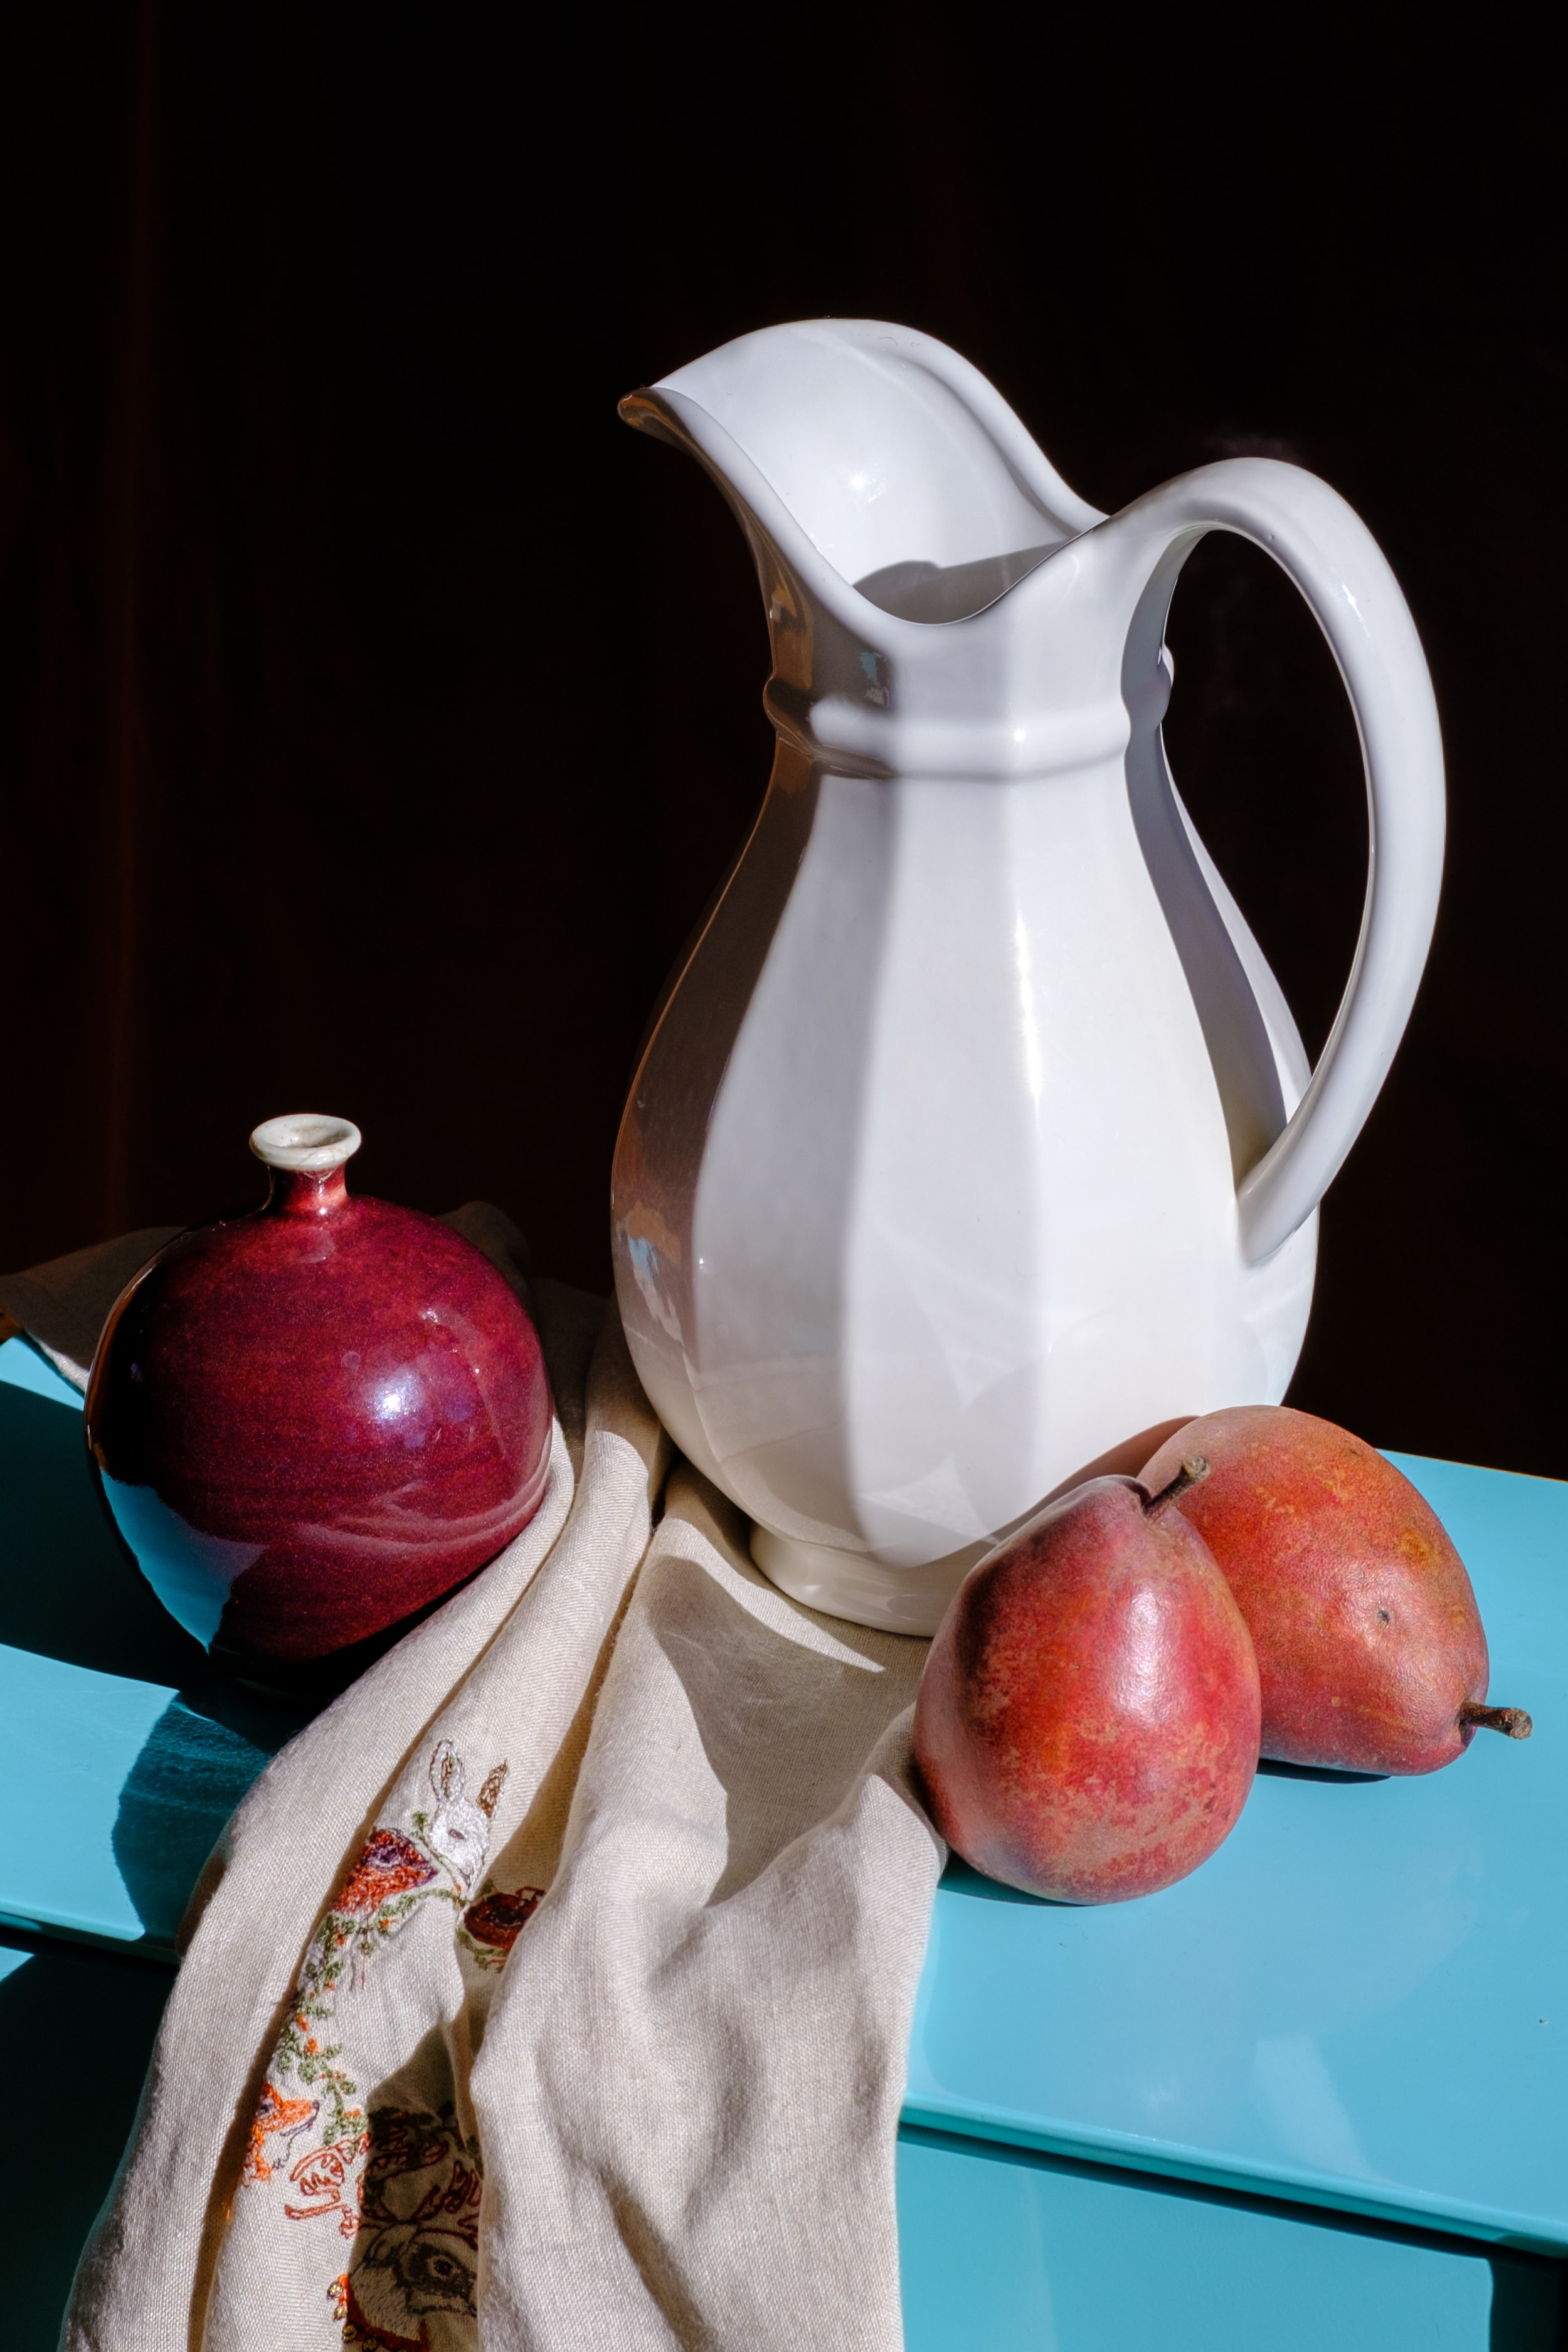
\includegraphics[width=\linewidth]{../images/2.jpg}
  \caption*{2.jpg}
  \label{fig:2jpg}
\end{subfigure}

\medskip
\begin{subfigure}{0.25\textwidth}
  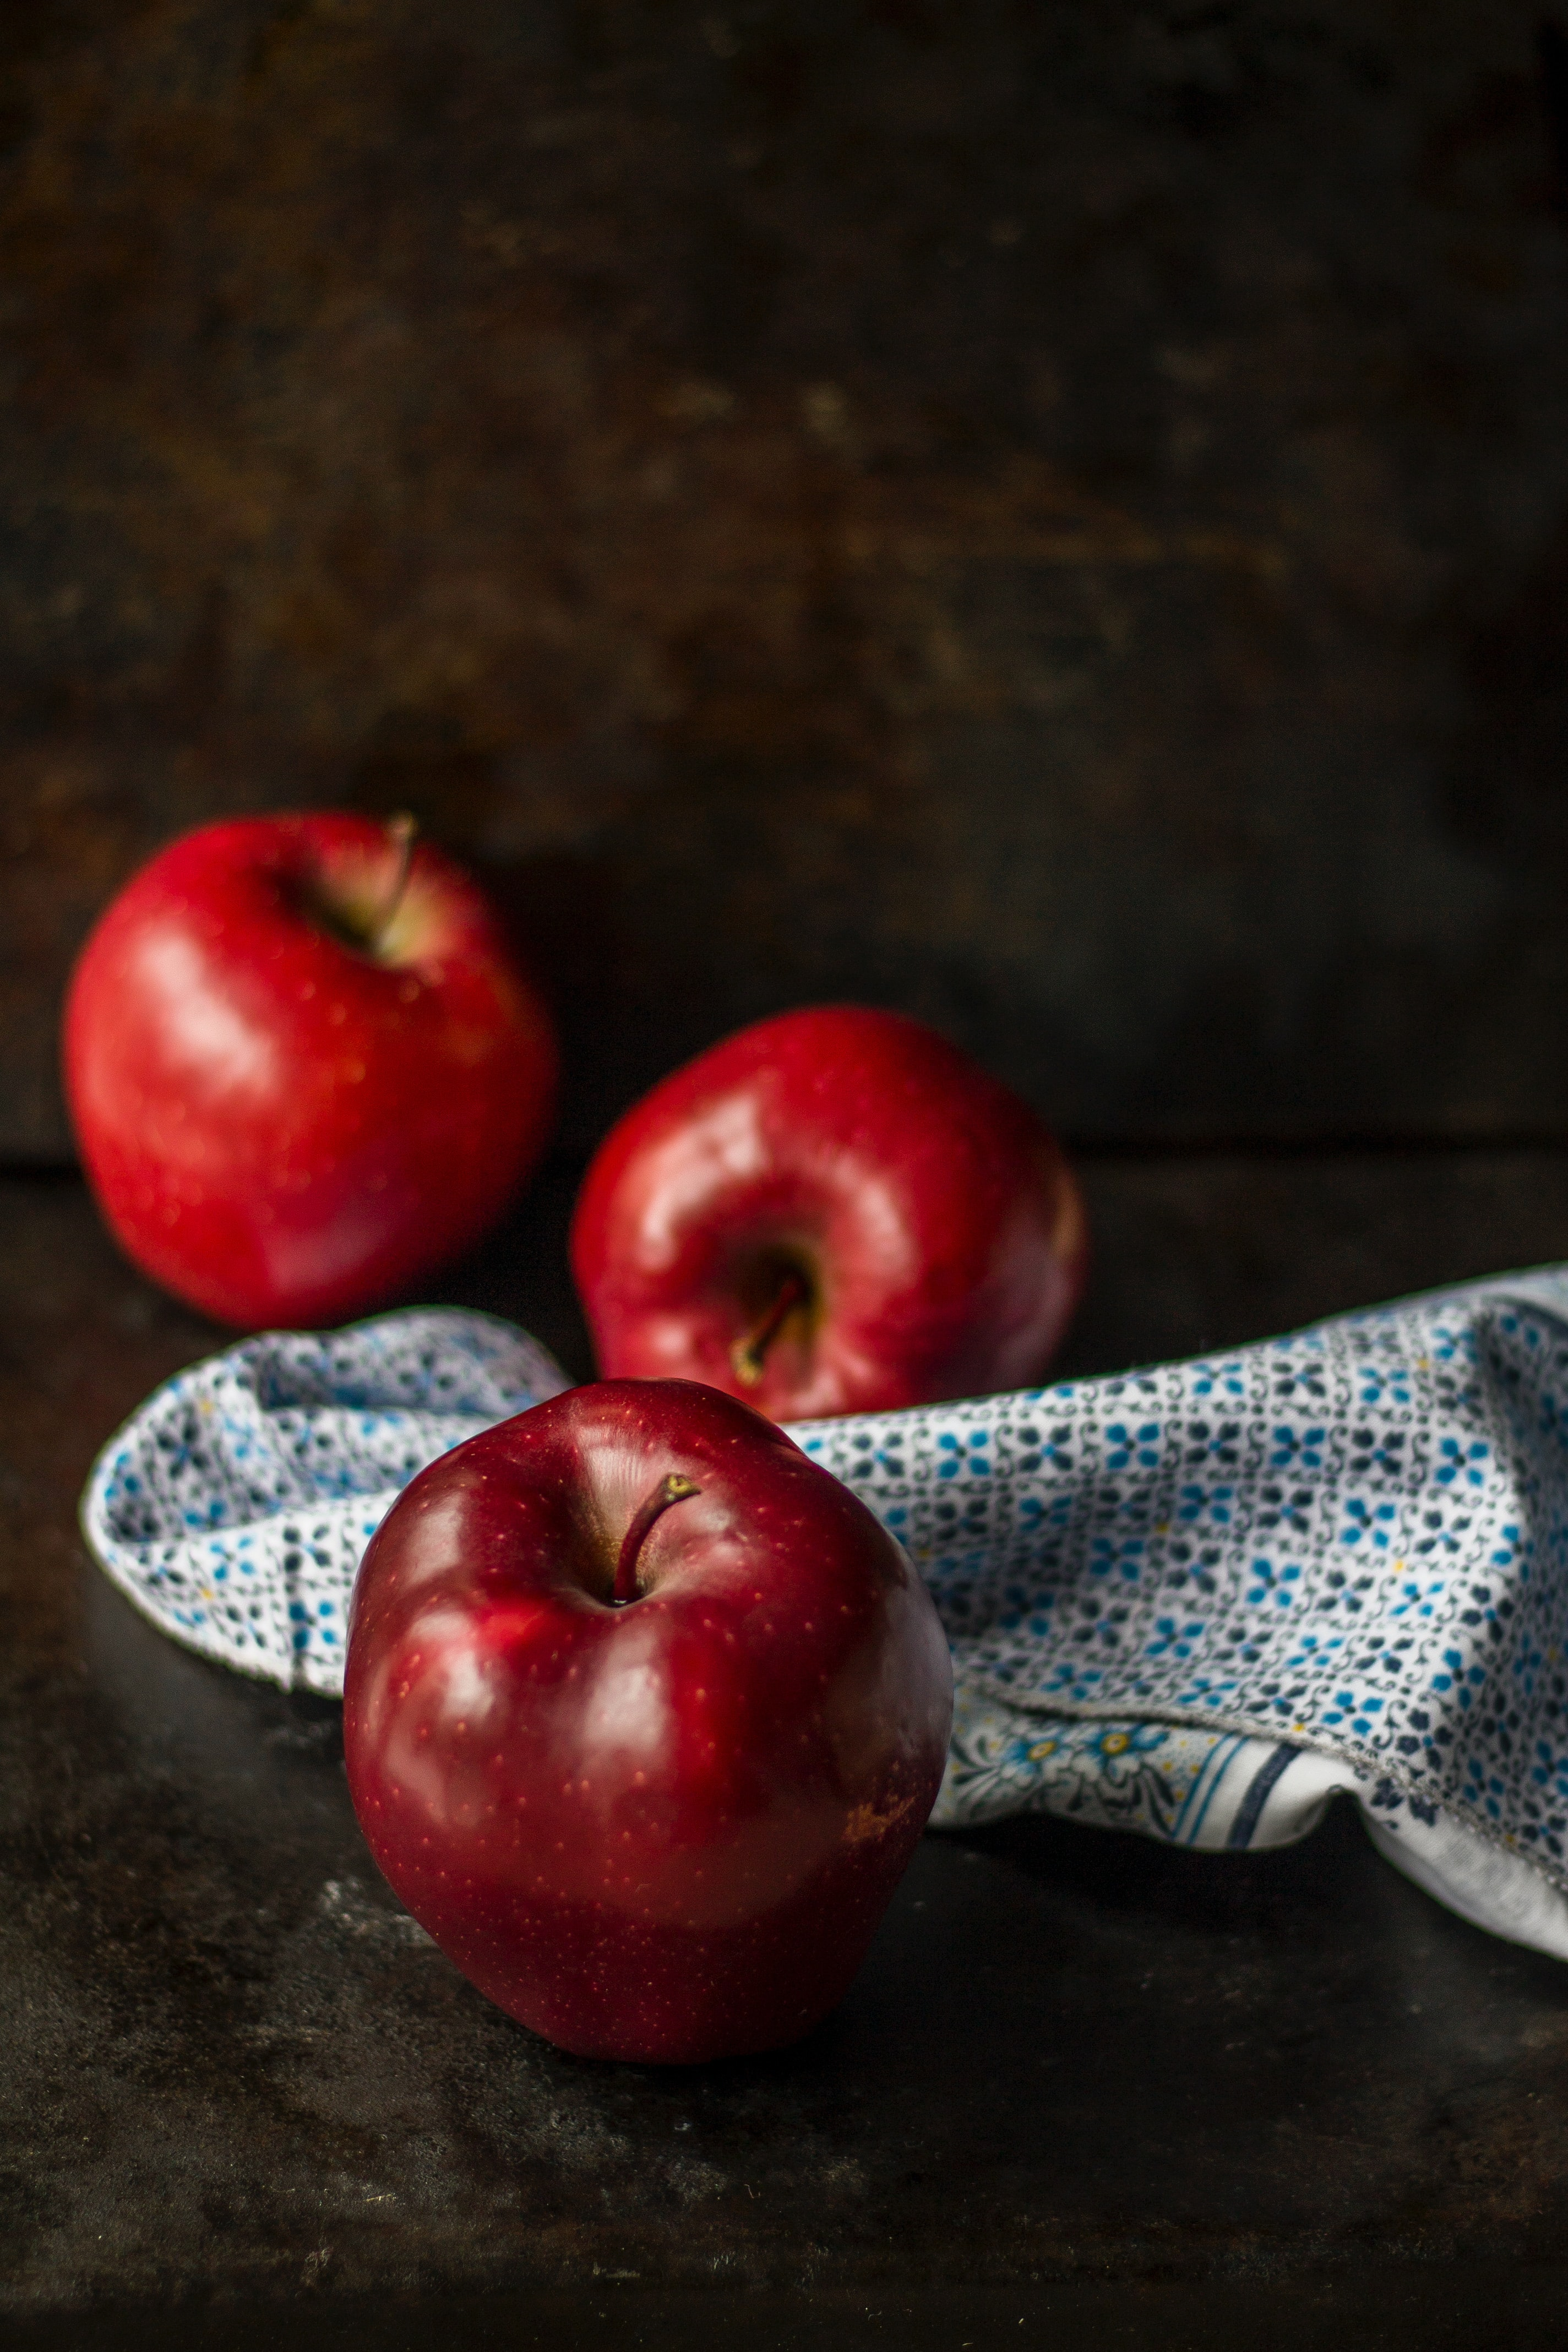
\includegraphics[width=\linewidth]{../images/3.jpg}
  \caption*{3.jpg}
  \label{fig:3jpg}
\end{subfigure}\hfil % <-- added
\begin{subfigure}{0.25\textwidth}
  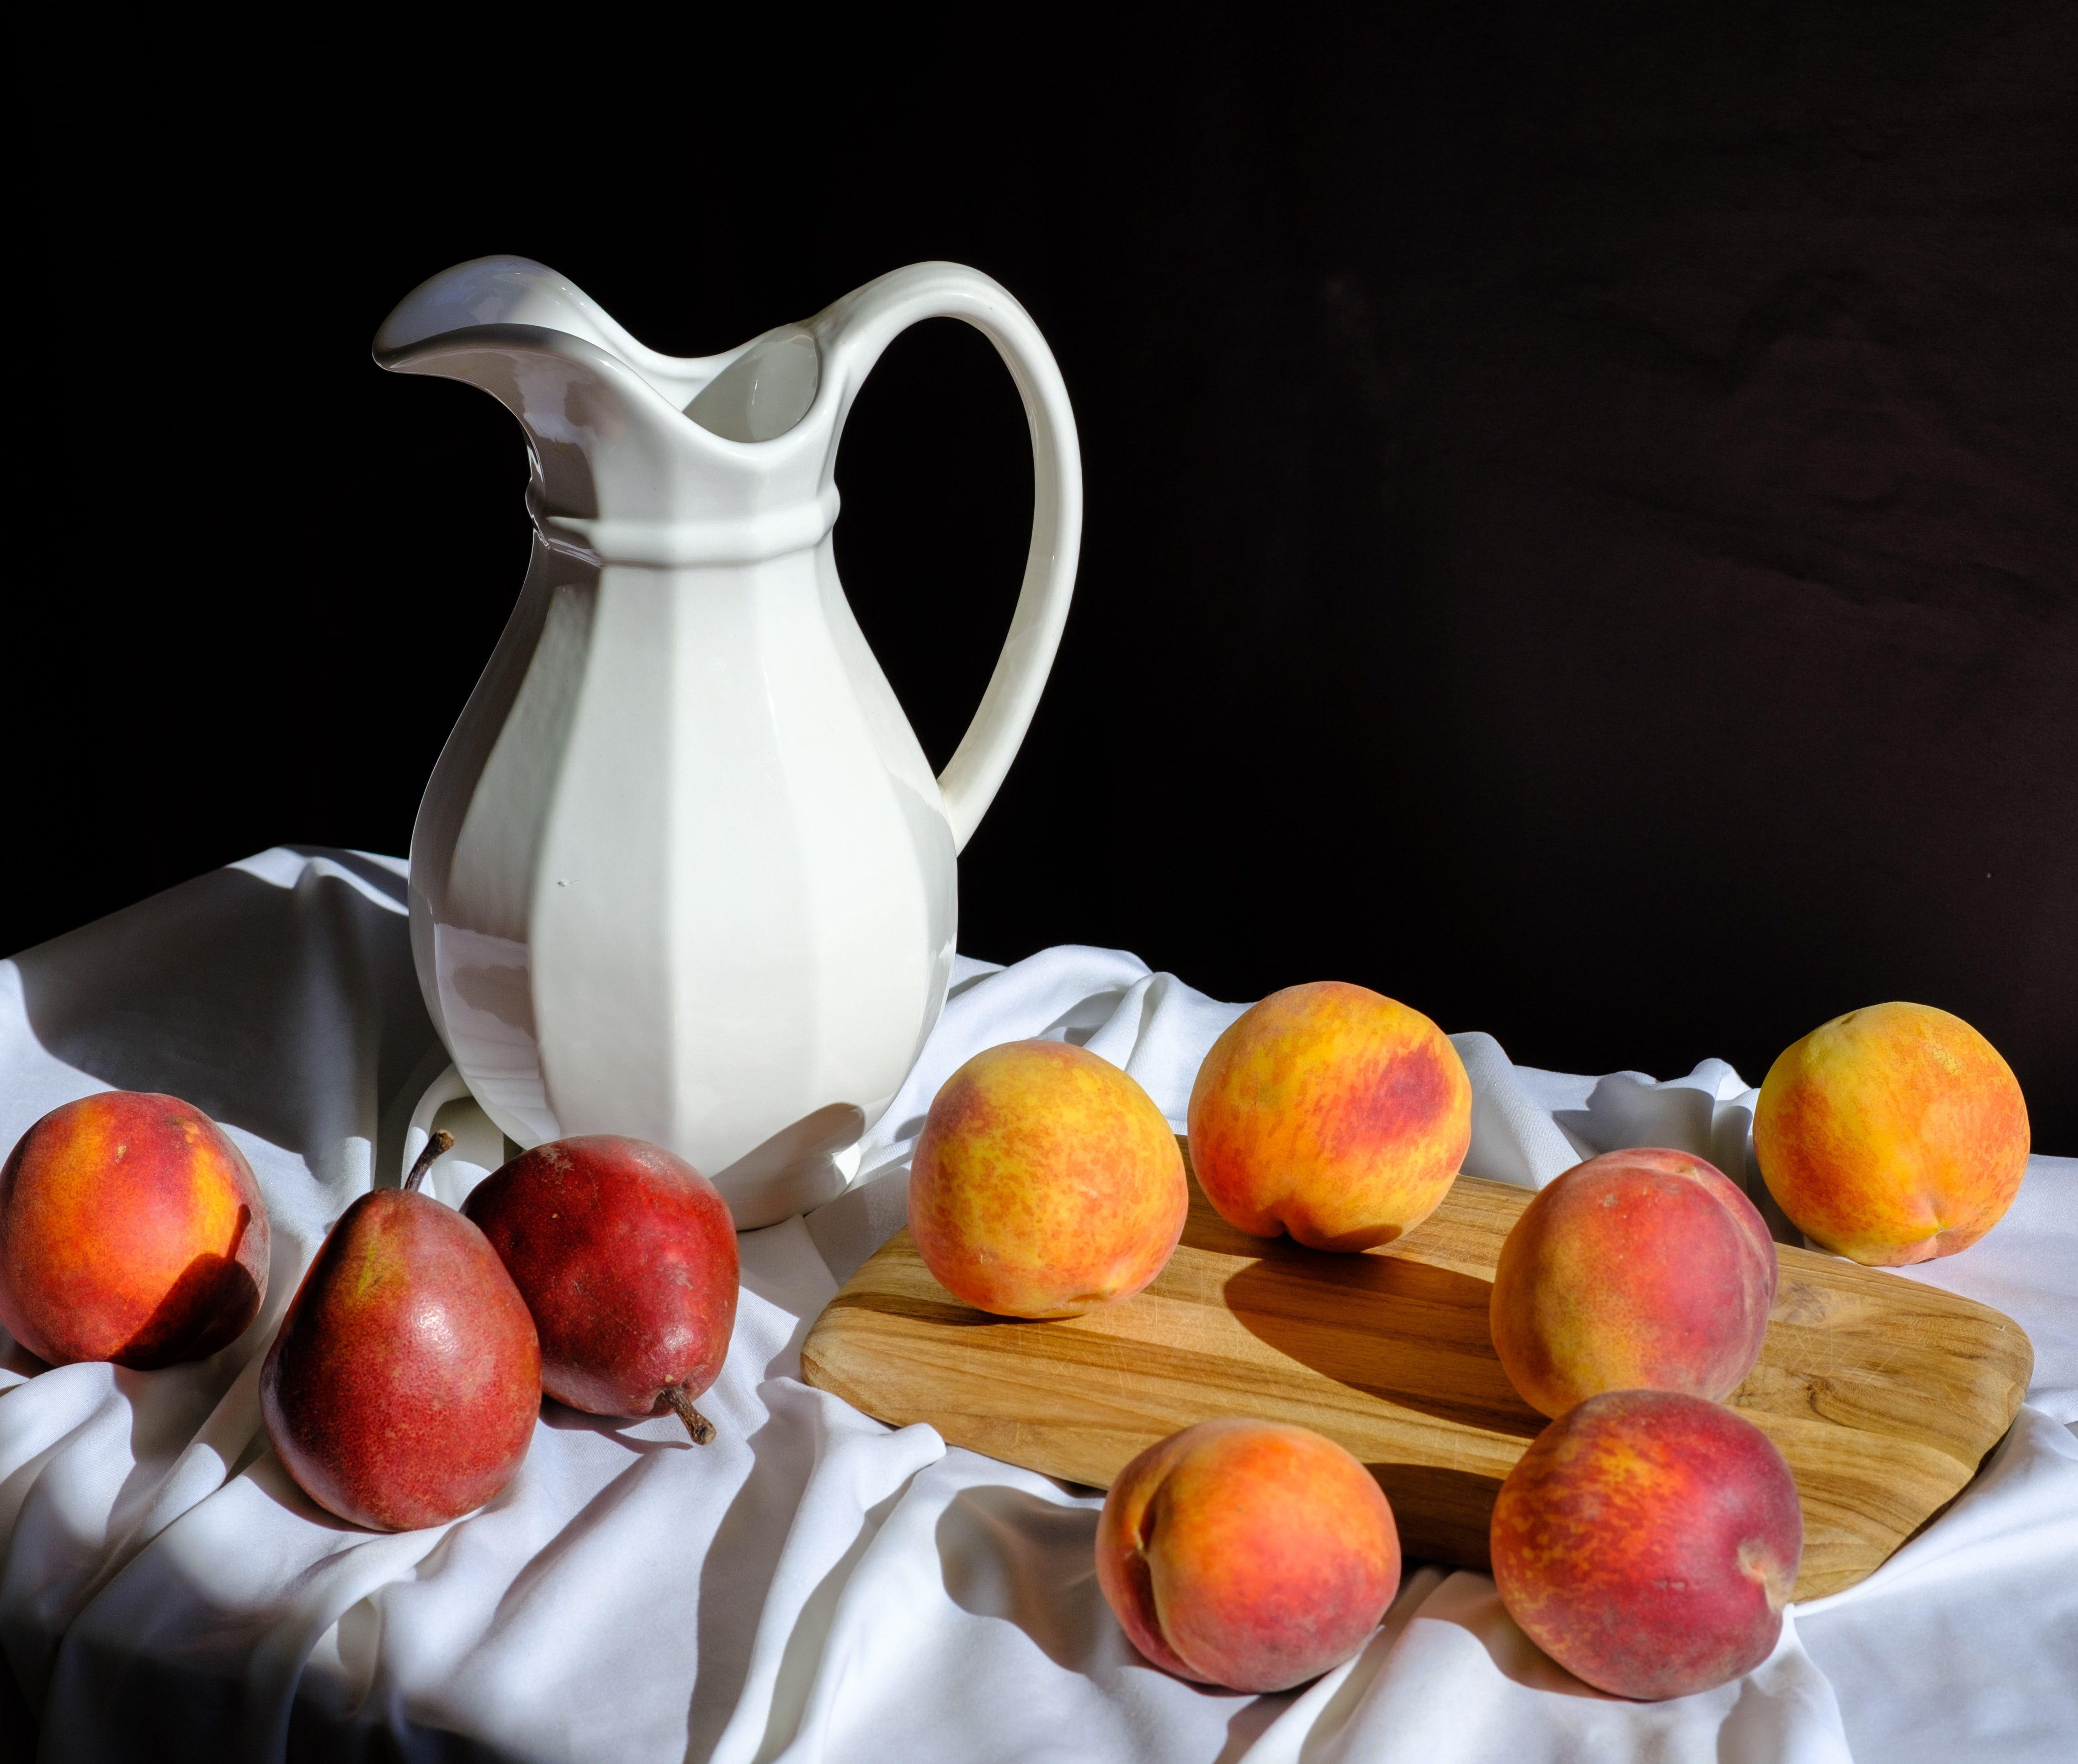
\includegraphics[width=\linewidth]{../images/4.jpg}
  \caption*{4.jpg}
  \label{fig:4jpg}
\end{subfigure}\hfil % <-- added
\begin{subfigure}{0.25\textwidth}
  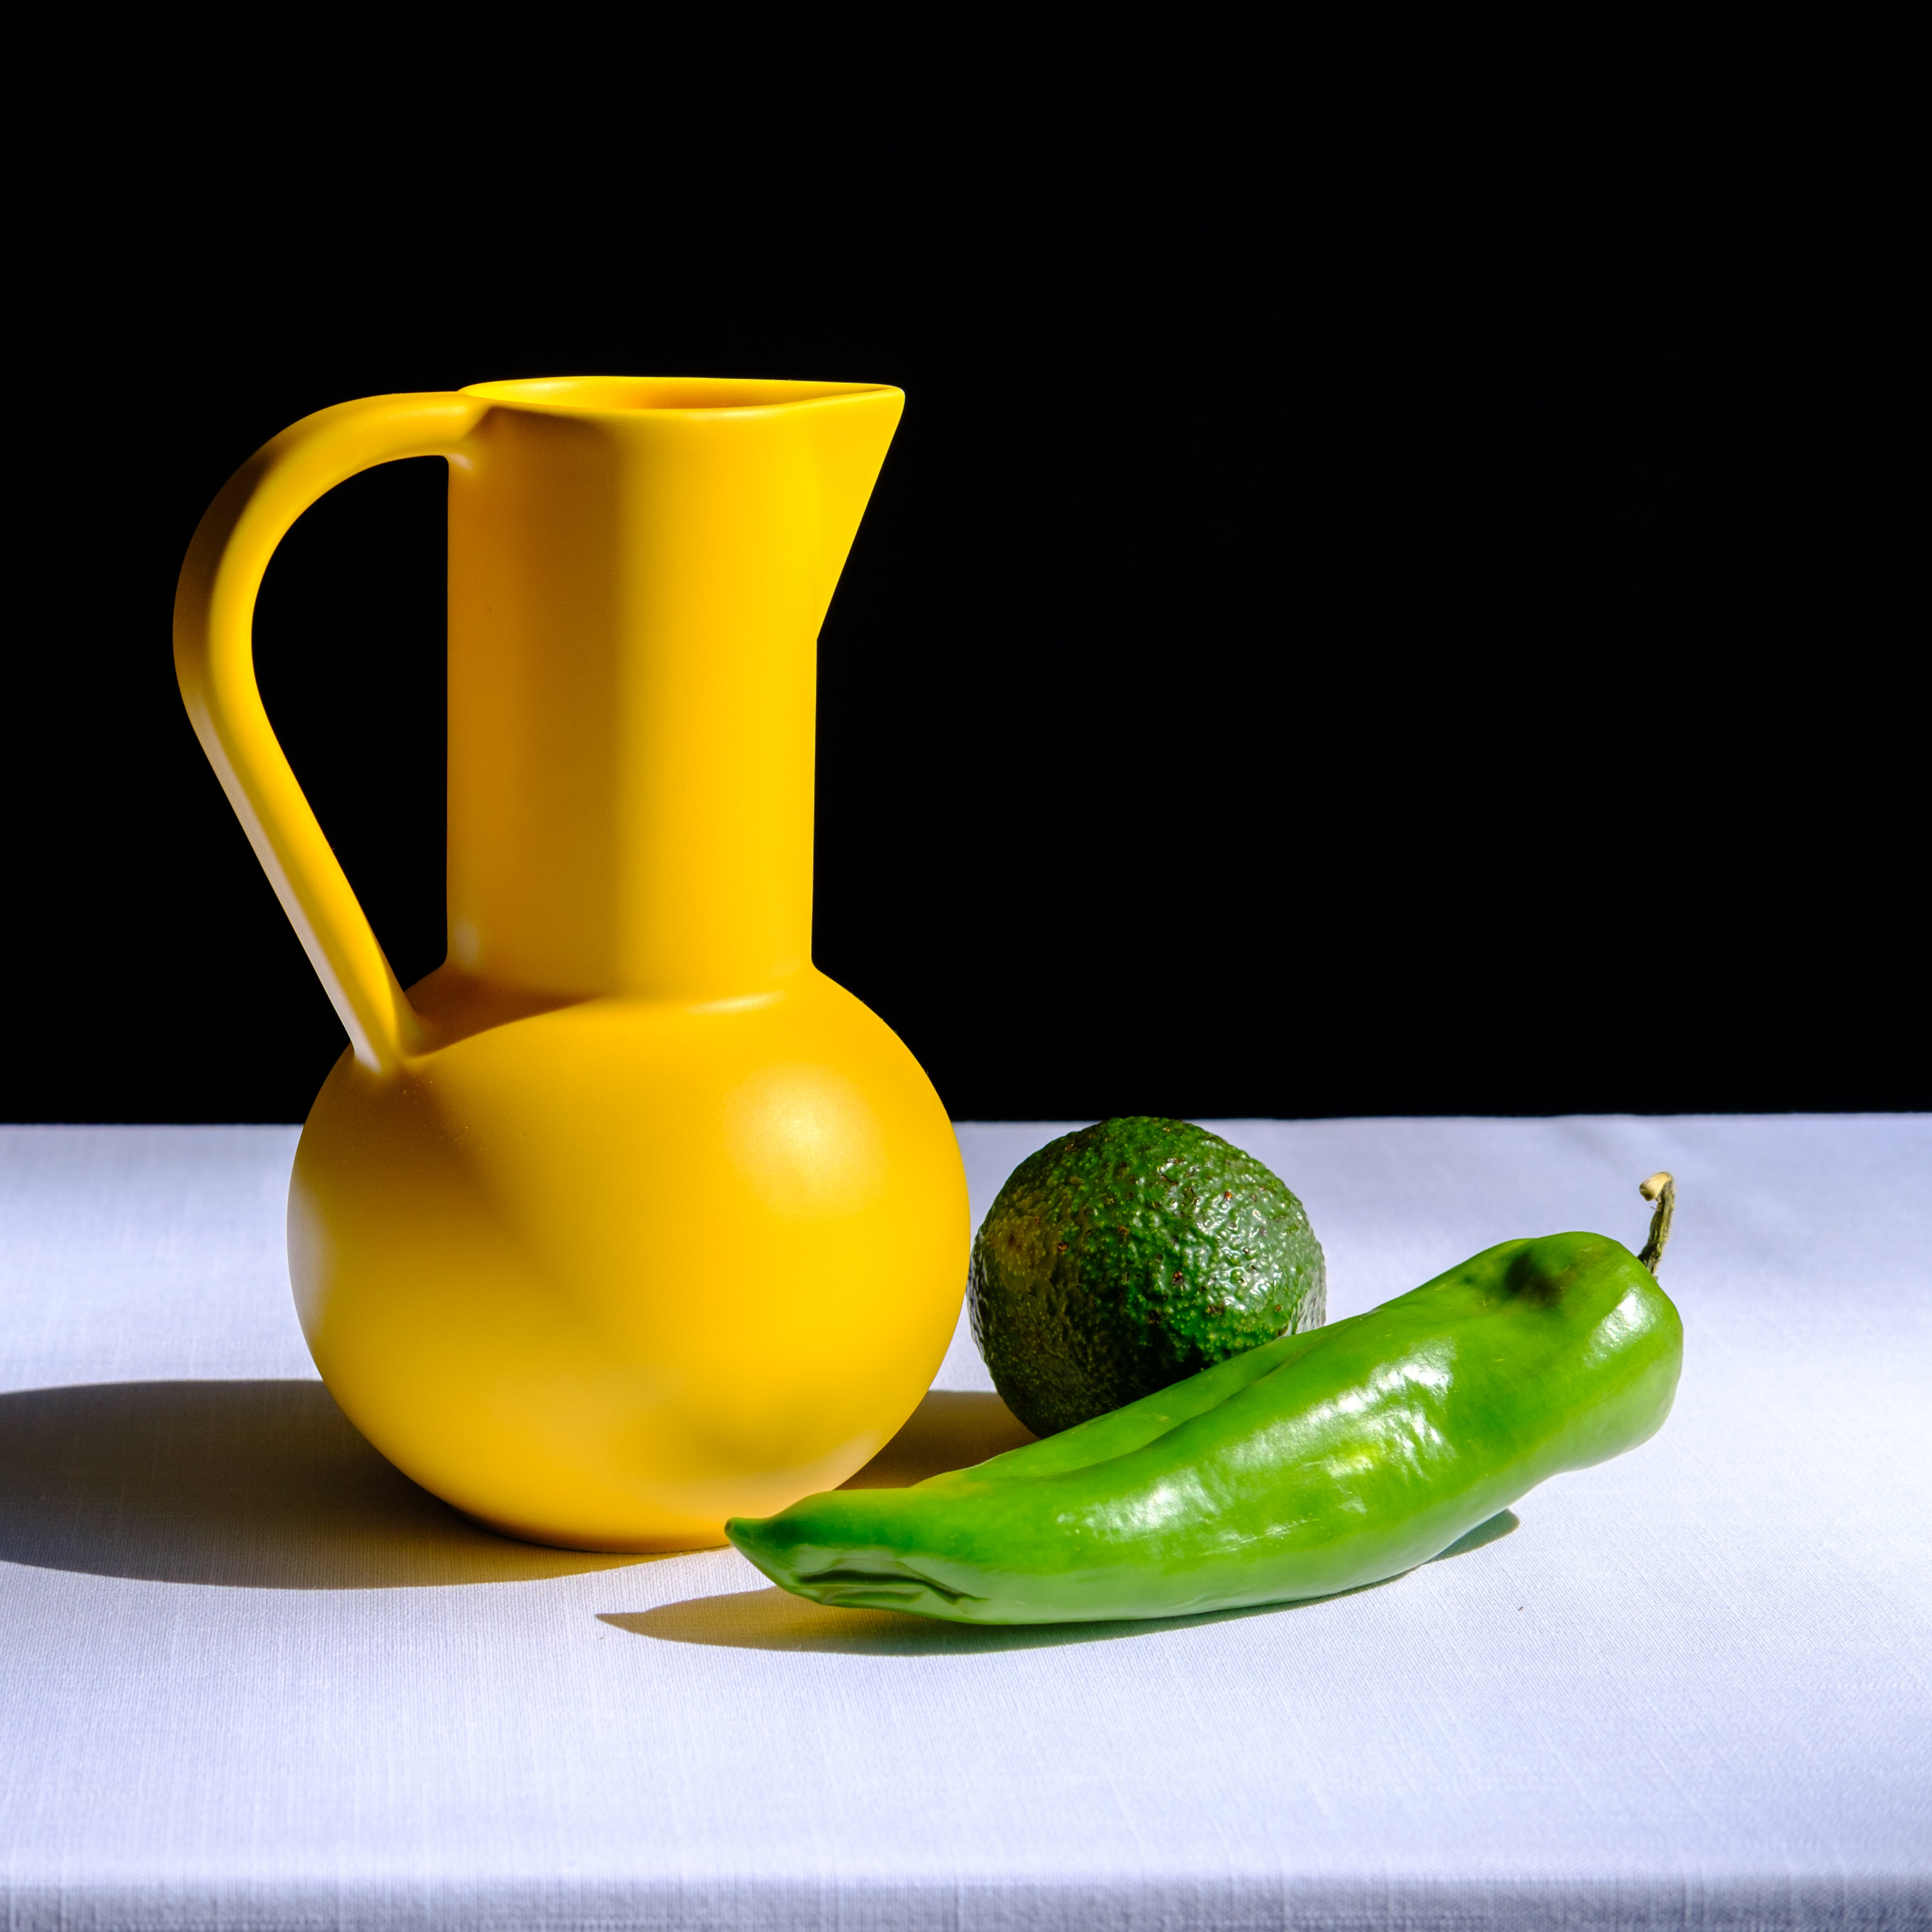
\includegraphics[width=\linewidth]{../images/5.jpg}
  \caption*{5.jpg}
  \label{fig:5jpg}
\end{subfigure}
\caption{Felhasznált képek}
\label{fig:images}
\end{figure}

\Section{Képek feldolgozása}

A képek feldolgozása során előfordulnak olyan lépések, műveletek amelyeket több ponton is megismételtem. Ezeket ebben a bekezdésben szeretném bemutatni, a későbbiekben nem térek ki rájuk részletesen.
A képfeldolgozáshoz az \texttt{opencv-python} könyvtárat használtam.

\SubSection{Betöltés}

A képeket két módon töltöm be a további feldolgozásra:
\begin{itemize}
\item színesen
\item szürkeárnyalatosan
\end{itemize}
Ehhez két külön metódust készítettem:
\begin{itemize}
\item \texttt{load\_image\_rgb}
\item \texttt{load\_image\_grayscale}
\end{itemize}
Ezek eleinte minden munkafüzetben ismétlődtek, majd a kutatás későbbi szakaszában kiszerveztem őket a \texttt{commonmethods} nevű saját készítésű python librarybe amiről részletesebben a következő alfejezetben írok.

A szürkeárnyalatos kép betöltését a következő kódrészlet tartalmazza.
\begin{python}
import cv2

def load_image_grayscale(name):
    """
    Loading the image from the images folder using opencv-python
    :param name: the name of the image I want to load,
        the method doesn't need the path or the extension
    :return: the loaded image in grayscale color
    """
    image = cv2.imread('../images/' + format(name) + '.jpg')
    image = cv2.cvtColor(image, cv2.COLOR_BGR2GRAY)

    return image
\end{python}
A színes kép betöltése annyiban különbözik, hogy a cv2.COLOR\_BGR2GRAY helyett cv2.COLOR\_BGR2RGB szerepel.

Mind a két metódus a kép nevét várja bemenetként. Mivel a tesztelés során használt képek mindegyike JPG típusú, így a kiterjesztést a metódus automatikusan hozzákapcsolja.

\SubSection{Átméretezés}

Átméretezésre a \texttt{resize\_image} metódust készítettem, amelynek a forráskódja a következő:
\begin{python}
import cv2

def resize_image(image, desired_height) :
    """
    Resizing the image for the given height,
    without disortion, using opencv-python
    :param image: the image that I want to resize
    :param desired_height: the height in pixel that
        I want to have in the resized image
    :return: the resized image
    """
    height = image.shape[0]
    # calculating the amount with I need to change the width
    scale_percent = height / desired_height
    width = int(image.shape[1] / scale_percent)
    dim = (width, desired_height)

    resized_image = \
        cv2.resize(image, dim, interpolation = cv2.INTER_AREA)

    return resized_image
\end{python}
Bemenetként magát a képet várja és azt a méretet px-ben, amire a magasságot szeretnénk változtatni. Hogy ne torzuljon a kép, kiszámítok egy arányt a paraméterként kapott méretből és a kép magasságából, majd ezzel az aránnyal csökkentem a kép szélességét.

\Section{Közös metódusok kiszervezése}

Mint már az előző alfejezetekben említettem, több olyan metódus is előfordult, amit több python-notebook esetén is alkalmaztam. Eleinte csak átmásoltam egyik notebook-ból a másikba a kódot, de ahogy egyre többször ismétlődött ugyanaz a kódrész úgy döntöttem, hogy ideje kiszervezni őket.

Úgy nevezett Python Package-t, Python csomagot készítettem belőlük méghozzá azért, mert egyszerűen használható. A generálása után a \texttt{pip} parancs segítségével futtatható és ha szeretnénk, tudjuk ezeket publikálni is. \cite{pythonlibrary}

Ahhoz hogy létre tudjunk hozni egy ilyen csomagot, szükséges hogy a \texttt{pip} legfrissebb verziója legyen feltelepítve, ezen kívül szükségesek a \texttt{wheel} és a \texttt{setuptools} nevezetű könyvtárak.

Ha szeretnénk publikálni is a munkákat akkor azt a \texttt{twine} könyvtár segítségével tehetjük meg.

Első lépésként meg kell határoznunk a csomag nevét, érdemes minél rövidebb nevet választani hogy könnyen hivatkozható legyen. Én a \texttt{commonmethods} nevet választottam, mivel a csomag az általánosan használt metódusaimat fogja tartalmazni.

Ezután következik a struktúra felépítése ami nálam a következő:
\begin{python}
mycommonmethods/
|-- setup.py
|-- commonmethods/
	|-- __init__.py
	|-- image_modification.py
	|-- optimal_cluster_number.py
\end{python}
A fájlok a következőket tartalmazzák:
\begin{itemize}
\item \texttt{setup.py}: A setup.py a legfontosabb fájl a könyvtár készítése során, mivel ebben határozzuk meg a telepítési információkat.
\item \texttt{\_\_init\_\_.py}: Minden mappa ami tartalmaz init fájlt az belekerül a könyvtárunkba a buildelés során. A kód amit ide írunk, az az import során lefut, tehát csak minimális kódot érdemes beleírni. Általában üresen szokták hagyni, az én esetemben is üresen maradt.
\item \texttt{image\_modification.py}: Ebben a Python fájlban található meg minden olyan metódus, ami a képek módosításához kapcsolódik.
 \begin{sloppypar}
 A \texttt{load\_image\_rgb}, \texttt{load\_image\_grayscale} és a \texttt{resize\_image} metódusok már bemutatásra kerültek a fentebbi alfejezetekben.
 \end{sloppypar}
  Ezeken kívül még a \texttt{kmeans\_segmentation} nevezetű metódust tartalmazza, amiről a következő fejezetben írok bővebben.
\item \texttt{optimal\_cluster\_number.py}: Ebben a Python fájlban az optimális klaszterszám meghatározására használt metódusok találhatók. Részletes bemutatásukat a következő fejezet tartalmazza.
\end{itemize}

Általában teszt fájlokat is szoktak készíteni a csomag létrehozása során, én ezt a lépést kihagytam. Amennyiben szeretnénk ténylegesen publikálni a munkákat akkor viszont elengedhetetlen a tesztelés annak érdekében, hogy a kiadott verzióink minél stabilabbak legyenek.

Amint felépítettük a struktúránkat és elkészítettük a megfelelő fájlokat, ideje buildelni a könyvtárunkat. Ehhez a \texttt{setup.py} fájlt kell futtatnunk a következő parancs segítségével:
\begin{python}
python setup.py bdist_wheel
\end{python}

Ez generál nekünk egy \texttt{dist} nevű mappát amiben benne lesz egy \texttt{.whl} kiterjesztésű fájl. Ezt a fájlt kell futtassuk a következő módon:

\begin{python}
pip install /path/wheelfile.whl
\end{python}

A futtatás után már használható is a könyvtárunk, én a következő módon hivatkozok rá a notebookokban:
\begin{python}
import commonmethods.image_modification as im
import commonmethods.optimal_cluster_number as ocn
\end{python}

A fájlok listázása során említettem hogy a \texttt{setup.py} a legfontosabb mivel ennek alapján készül el a könyvtárunk, így ennek a tartalmát a következő alfejezetben szeretném részletesen bemutatni.

\SubSection{setup.py}

A \texttt{setup.py} fájl a scriptünk amit a \texttt{setuptools} fog használni hogy elkészítse a könyvtárat. Ebben található meg minden főbb információ a csomagunkról. A következő kódrészlet az én \texttt{setup.py} fájlom ami egy minimális készletet használ, ennél sokkal több argumentumot ismer a \texttt{setup()}. A teljes argumentum lista megtalálható a \cite{setup} oldalon.
\begin{python}
from setuptools import setup, find_packages

VERSION = '1.0.0'
DESCRIPTION = 'Python package for my diploma thesis'
LONG_DESCRIPTION = 'Python package for my diploma thesis that contains \
some common methods that I use in different python notebooks'

# Setting up
setup(
        name="commonmethods",
        version=VERSION,
        author="Fanni Molnar",
        author_email="<fannimolnr98@gmail.com>",
        description=DESCRIPTION,
        long_description=LONG_DESCRIPTION,
        packages=find_packages(),
        install_requires=['scikit-learn', 'numpy', 'opencv-python']
)
\end{python}
Az argumentumokról részletesebben:
\begin{itemize}
\item \texttt{name}: Ezen a néven tudjuk majd hivatkozni a könyvtárunkat. Csak betűket, számokat, \_, és - karaktereket tartalmazhat. Amennyiben szeretnénk publikálni a csomagunkat, akkor egyedinek kell lennie a pypi.org oldalon.
\item \texttt{version}: A csomagunk verziója.
\item \texttt{author} és \texttt{author\_email}: A készítő adatai.
\item \texttt{description}: Rövid, egy mondatos leírás ami összefoglalja a csomag tartalmát.
\item \texttt{long\_description}: Részletes leírása a csomagnak, gyakran használják úgy hogy a \texttt{README.md} fájlból töltik be.
\item \texttt{packages}: Itt tudjuk megadni, hogy mely csomagokat szeretnénk hozzáadni a könyvtárunkhoz. Egyszerűen használhatjuk a \texttt{find\_packages()} metódust ami automatikusan megtalálja a csomagokat. Az én esetemben az egyedüli csomag a \texttt{commonmethods}.
\item \texttt{install\_requires}: Itt tudjuk megadni hogy a csomagunk használatához milyen könyvtárak szükségesek. Amennyiben valamelyik csomag hiányzik, azt a telepítés elején automatikusan feltelepíti, ezért itt minden esetben csak az elengedhetetlen könyvtárakat adjuk meg.
\end{itemize}

\Section{Tesztelési környezet}

A programkódok tesztelését minden esetben az otthoni számítógépemen végeztem aminek a paraméterei a következők:
\begin{itemize}
\item Processzor: Intel(R) Core(TM) i5-9400F CPU 2.90GHz
\item Memória mérete: 16 GB
\item Videókártya: NVIDIA GeForce GTX 1660
\item Operációs rendszer: Windows 10 Enterprise
\end{itemize} 